\documentclass{jsarticle}
\usepackage[dvipdfmx,hiresbb]{graphicx}
\begin{document}

\section{通常}
画像\texttt{tiger1.pdf} が読み込まれる。

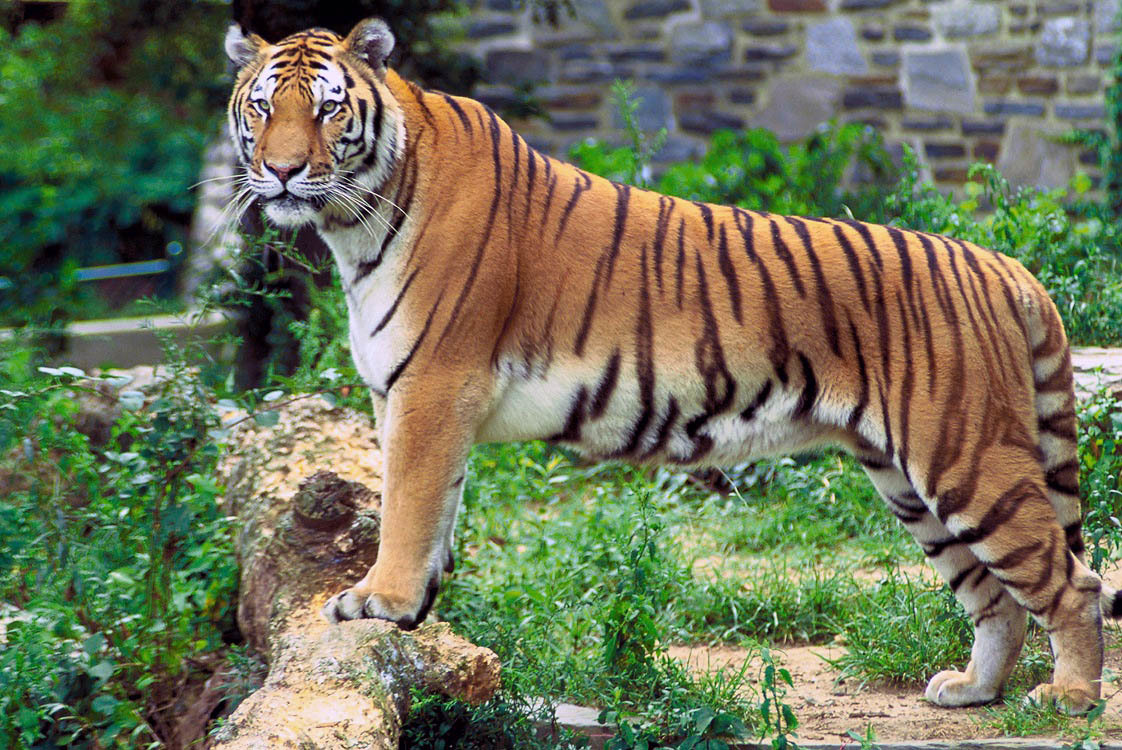
\includegraphics[width=15cm]{tiger1.pdf}

\section{行頭からのコメント}
コメント内の画像\texttt{tiger2.pdf} は読み込まれない。

% 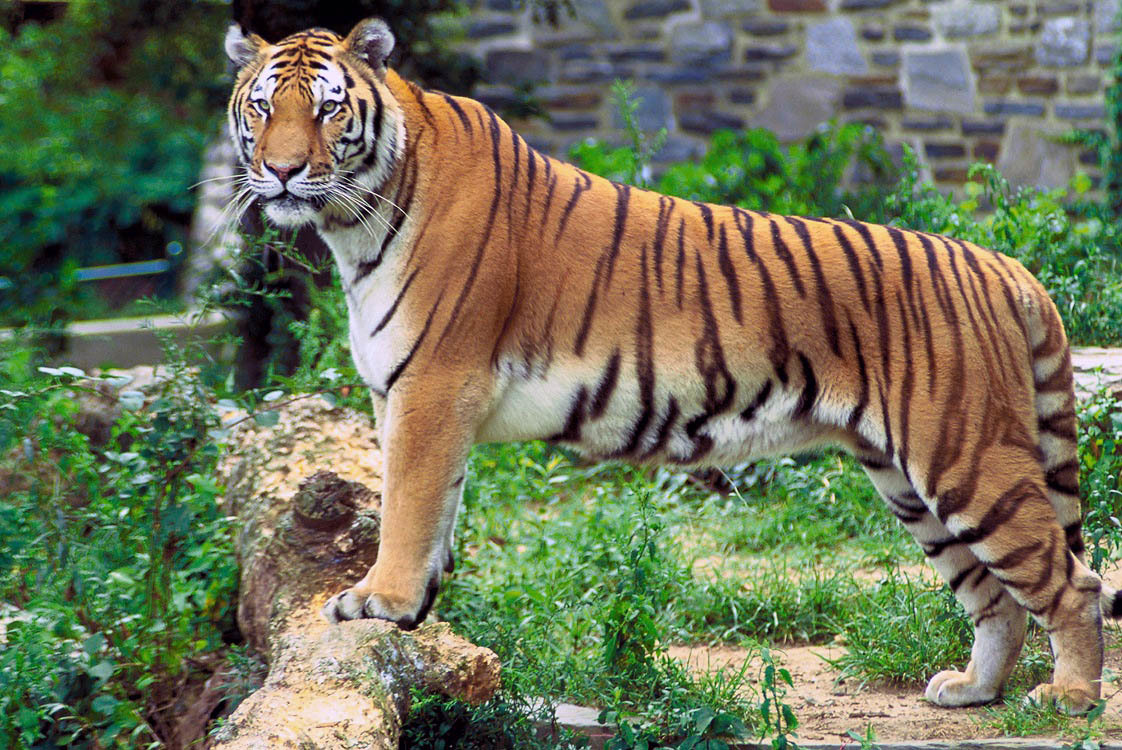
\includegraphics[width=15cm]{tiger2.pdf}

\section{行の途中でコメント}
コメント内の画像\texttt{tiger3.pdf} は読み込まれてはならない。% 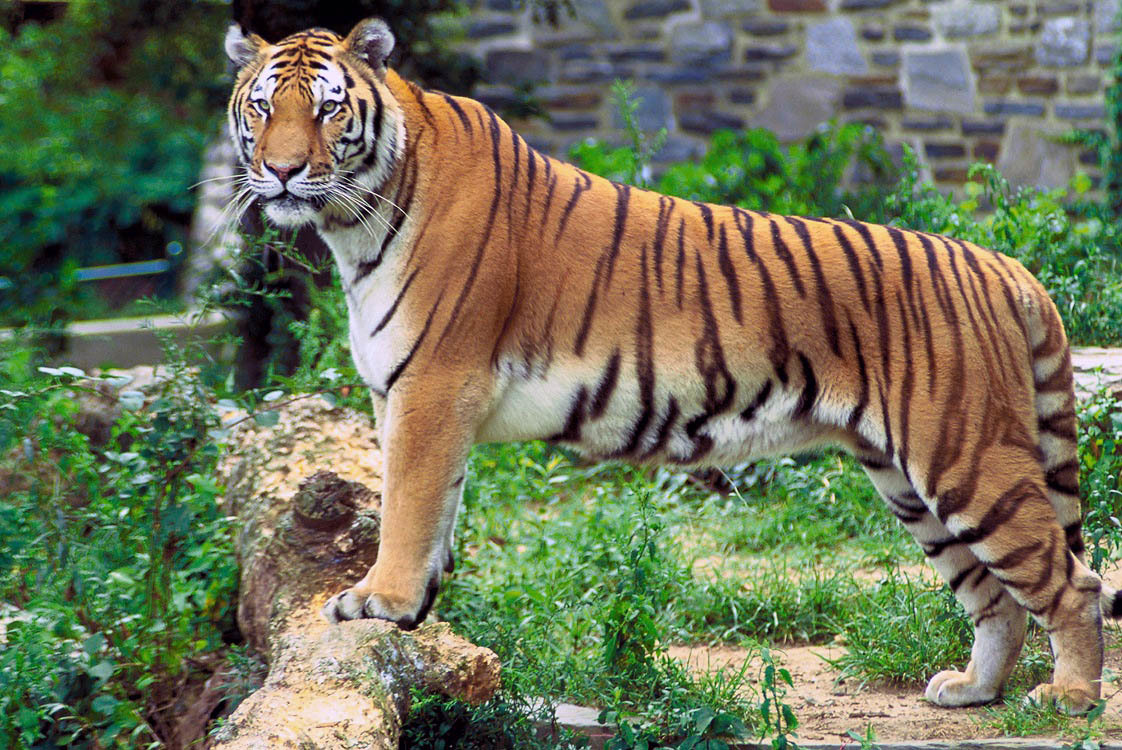
\includegraphics[width=15cm]{tiger3.pdf}

\section[行中に\%を挿入]{行中に\texttt{$\backslash$\%} を挿入}
\verb|\%| の後に記載された画像\texttt{tiger4.pdf} は読み込まれる。

\% 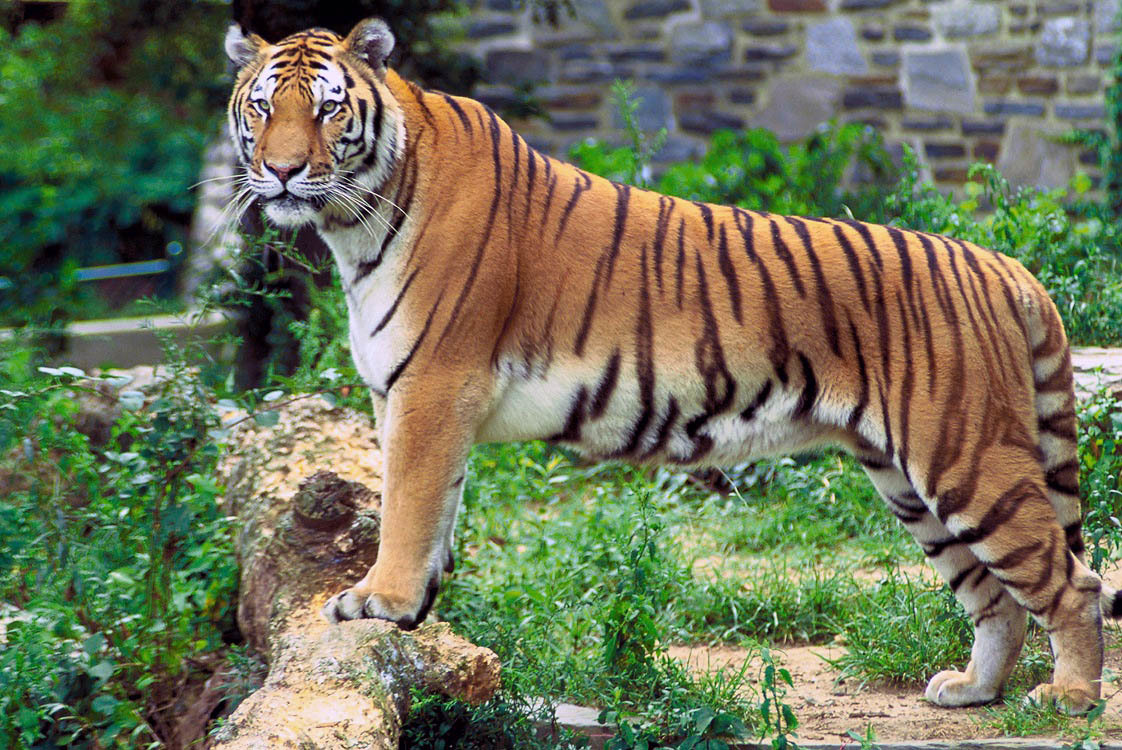
\includegraphics[width=15cm]{tiger4.pdf}

\section{\tt{verbatim}環境}
\texttt{verbatim}環境内の画像\texttt{tiger5.pdf} は読み込まれない。

\begin{verbatim}
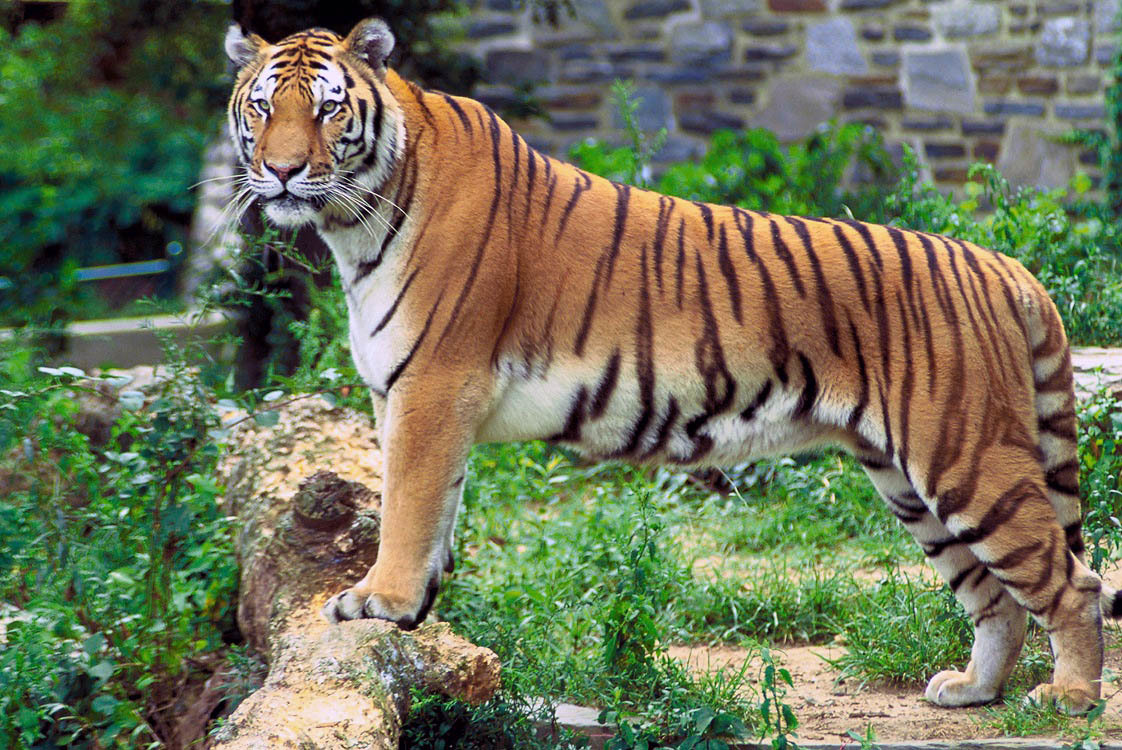
\includegraphics[width=15cm]{tiger5.pdf}
\end{verbatim}
\end{document}
